\documentclass{standalone}
\usepackage{float}
\usepackage{tikz}
\usepackage{lmodern}
\usepackage{amsmath}
\usetikzlibrary{calc}
\usetikzlibrary{decorations.markings}
\usetikzlibrary{patterns, patterns.meta}

\begin{document}

\centering

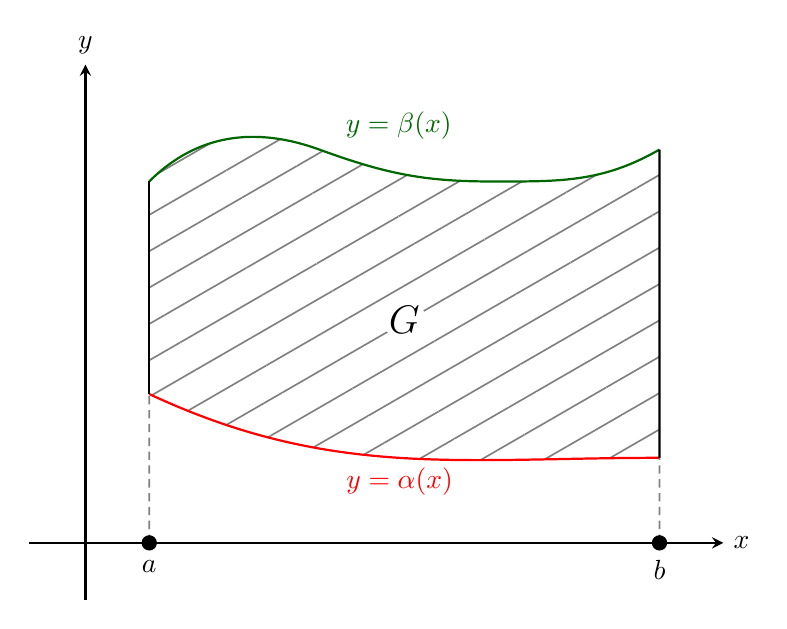
\begin{tikzpicture}[scale=0.9]
\pgfmathsetmacro{\CircleSize}{0.09}     % radius of coordinate circles/dots
% define styles used in this picture
\tikzset{BigTextFont/.style={font=\Large},
every node/.style={font=\normalsize, text=black},
CircleNodeStyle/.style={draw=black, shape=circle, fill=black, minimum size=\CircleSize*2 cm, inner sep=0pt},
arrowstyle/.style={->, >=stealth}}

% custom colors
\definecolor{Green}{rgb}{0.0, 0.4, 0.0}
\definecolor{Red}{rgb}{1, 0, 0}

% axes
\pgfmathsetmacro{\OvershootAxis}{0.8}

\draw[arrowstyle, thick] (-\OvershootAxis,0) -- (9,0) node[pos=1, right] {$x$};
\draw[arrowstyle, thick] (0,-\OvershootAxis) -- (0,6.75) node[pos=1, above] {$y$};

% defining smooth curve 1:
\coordinate (Begin1) at (0.9, 5.1);
\coordinate (Bend1) at ($(Begin1)+(2.4, 0.45)$);
\coordinate (FlatMid1) at ($(Bend1)+(2.4, -0.45)$);
\coordinate (End1) at ($(FlatMid1) + (2.4, 0.45)$);
% define in and out angles
\pgfmathsetmacro{\OutAngleAA}{45}
\pgfmathsetmacro{\InAngleAA}{160}
\pgfmathsetmacro{\OutAngleAB}{-20}
\pgfmathsetmacro{\InAngleAB}{180}
\pgfmathsetmacro{\OutAngleAC}{0}
\pgfmathsetmacro{\InAngleAC}{210}

% defining smooth curve 2:
\coordinate (Begin2) at (0.9, 2.1);
\coordinate (End2) at ($(Begin2) + (7.2, -0.9)$);
\pgfmathsetmacro{\OutAngleBA}{335}
\pgfmathsetmacro{\InAngleBA}{180}

% apply pattern to area
\coordinate (CenterArea) at ($(Begin1)!0.5!(End2)$);
\fill[pattern={Lines[angle=30, distance=0.4cm, line width=0.6pt]}, pattern color=gray] (Begin1) to[out=\OutAngleAA, in=\InAngleAA] (Bend1) to[out=\OutAngleAB, in=\InAngleAB] (FlatMid1) to[out=\OutAngleAC, in=\InAngleAC] (End1) -- (End2) to[out=\InAngleBA, in=\OutAngleBA] (Begin2) -- cycle;
\node at (CenterArea) [draw=white, circle, inner sep=0, fill=white, BigTextFont] {$G$};

% draw smooth curve 1:
\draw[postaction={decorate}, decoration={
       markings,
       mark=at position 0.50 with {\node[above, yshift=0.3cm, text=Green] {$y=\beta(x)$};}}]
[Green, thick] (Begin1) to[out=\OutAngleAA, in=\InAngleAA] (Bend1) to[out=\OutAngleAB, in=\InAngleAB] (FlatMid1) to[out=\OutAngleAC, in=\InAngleAC] (End1);

% draw smooth curve 2:
\draw[postaction={decorate}, decoration={
       markings,
       mark=at position 0.50 with {\node[below, text=Red] {$y=\alpha(x)$};}}]
[thick, Red] (Begin2) to[out=\OutAngleBA, in=\InAngleBA] (End2);

% vertical sides
\draw[black, thick] (Begin1) -- (Begin2);
\draw[black, thick] (End1) -- (End2);

% dashed lines to domain
\draw[gray, semithick, densely dashed] (0.9,0) -- (Begin2);
\draw[gray, semithick, densely dashed] (8.1,0) -- (End2);
\node [CircleNodeStyle, label=below:$a$] at (0.9,0) {};
\node [CircleNodeStyle, label=below:$b$] at (8.1,0) {};

\end{tikzpicture}

\end{document}